\begin{figure}[htbp]
	\centering
	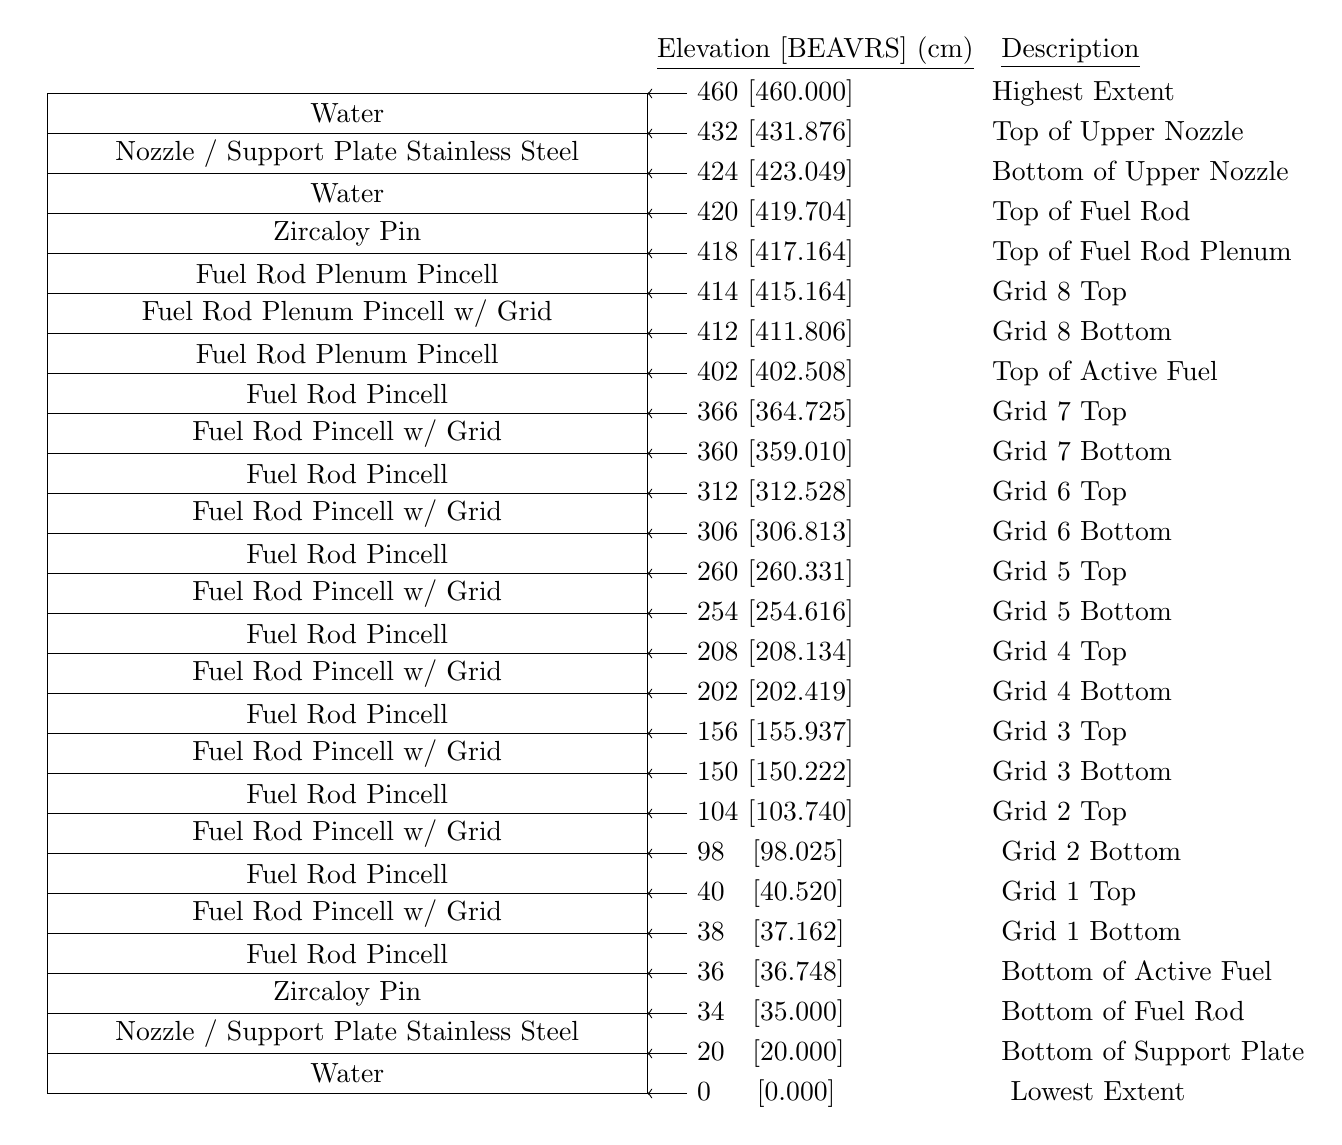
\begin{tikzpicture}[scale=1,x=1in,y=1in]
	\node[inner sep=0pt,
	text width=3 in,
	minimum size=0.2 in,
	draw=black,
	align=center,
	shift={(0,0.0)}] (n0) {Water};
	\draw[->] (1.7,-0.1) node[right,anchor=west] {0~~~~ [0.000] ~~~~~~~~~~~~~~~~~ Lowest Extent} -- (1.5,-0.1);
	\node[anchor=east] (s0) at (n0.west) {};
	\node[inner sep=0pt,
	text width=3 in,
	minimum size=0.2 in,
	draw=black,
	align=center,
	shift={(0,0.2)}] (n1) {Nozzle / Support Plate Stainless Steel};
	\draw[->] (1.7,0.1) node[right,anchor=west] {20~~ [20.000] ~~~~~~~~~~~~~~~ Bottom of Support Plate} -- (1.5,0.1);
	\node[inner sep=0pt,
	text width=3 in,
	minimum size=0.2 in,
	draw=black,
	align=center,
	shift={(0,0.4)}] (n2) {Zircaloy Pin};
	\draw[->] (1.7,0.3) node[right,anchor=west] {34~~ [35.000] ~~~~~~~~~~~~~~~ Bottom of Fuel Rod} -- (1.5,0.3);
	\node[inner sep=0pt,
	text width=3 in,
	minimum size=0.2 in,
	draw=black,
	align=center,
	shift={(0,0.6)}] (n3) {Fuel Rod Pincell};
	\draw[->] (1.7,0.5) node[right,anchor=west] {36~~ [36.748] ~~~~~~~~~~~~~~~ Bottom of Active Fuel} -- (1.5,0.5);
	\node[inner sep=0pt,
	text width=3 in,
	minimum size=0.2 in,
	draw=black,
	align=center,
	shift={(0,0.8)}] (n4) {Fuel Rod Pincell w/ Grid};
	\draw[->] (1.7,0.7) node[right,anchor=west] {38~~ [37.162] ~~~~~~~~~~~~~~~ Grid 1 Bottom} -- (1.5,0.7);
	\node[inner sep=0pt,
	text width=3 in,
	minimum size=0.2 in,
	draw=black,
	align=center,
	shift={(0,1.0)}] (n5) {Fuel Rod Pincell};
	\draw[->] (1.7,0.9) node[right,anchor=west] {40~~ [40.520] ~~~~~~~~~~~~~~~ Grid 1 Top} -- (1.5,0.9);
	\node[inner sep=0pt,
	text width=3 in,
	minimum size=0.2 in,
	draw=black,
	align=center,
	shift={(0,1.2)}] (n6) {Fuel Rod Pincell w/ Grid};
	\draw[->] (1.7,1.1) node[right,anchor=west] {98~~ [98.025] ~~~~~~~~~~~~~~~ Grid 2 Bottom} -- (1.5,1.1);
	\node[inner sep=0pt,
	text width=3 in,
	minimum size=0.2 in,
	draw=black,
	align=center,
	shift={(0,1.4)}] (n7) {Fuel Rod Pincell};
	\draw[->] (1.7,1.3) node[right,anchor=west] {104 [103.740] ~~~~~~~~~~~~~ Grid 2 Top} -- (1.5,1.3);
	\node[inner sep=0pt,
	text width=3 in,
	minimum size=0.2 in,
	draw=black,
	align=center,
	shift={(0,1.6)}] (n8) {Fuel Rod Pincell w/ Grid};
	\draw[->] (1.7,1.5) node[right,anchor=west] {150 [150.222] ~~~~~~~~~~~~~ Grid 3 Bottom} -- (1.5,1.5);
	\node[inner sep=0pt,
	text width=3 in,
	minimum size=0.2 in,
	draw=black,
	align=center,
	shift={(0,1.8)}] (n9) {Fuel Rod Pincell};
	\draw[->] (1.7,1.7) node[right,anchor=west] {156 [155.937] ~~~~~~~~~~~~~ Grid 3 Top} -- (1.5,1.7);
	\node[inner sep=0pt,
	text width=3 in,
	minimum size=0.2 in,
	draw=black,
	align=center,
	shift={(0,2.0)}] (n10) {Fuel Rod Pincell w/ Grid};
	\draw[->] (1.7,1.9) node[right,anchor=west] {202 [202.419] ~~~~~~~~~~~~~ Grid 4 Bottom} -- (1.5,1.9);
	\node[inner sep=0pt,
	text width=3 in,
	minimum size=0.2 in,
	draw=black,
	align=center,
	shift={(0,2.2)}] (n11) {Fuel Rod Pincell};
	\draw[->] (1.7,2.1) node[right,anchor=west] {208 [208.134] ~~~~~~~~~~~~~ Grid 4 Top} -- (1.5,2.1);
	\node[inner sep=0pt,
	text width=3 in,
	minimum size=0.2 in,
	draw=black,
	align=center,
	shift={(0,2.4)}] (n12) {Fuel Rod Pincell w/ Grid};
	\draw[->] (1.7,2.3) node[right,anchor=west] {254 [254.616] ~~~~~~~~~~~~~ Grid 5 Bottom} -- (1.5,2.3);
	\node[inner sep=0pt,
	text width=3 in,
	minimum size=0.2 in,
	draw=black,
	align=center,
	shift={(0,2.6)}] (n13) {Fuel Rod Pincell};
	\draw[->] (1.7,2.5) node[right,anchor=west] {260 [260.331] ~~~~~~~~~~~~~ Grid 5 Top} -- (1.5,2.5);
	\node[inner sep=0pt,
	text width=3 in,
	minimum size=0.2 in,
	draw=black,
	align=center,
	shift={(0,2.8)}] (n14) {Fuel Rod Pincell w/ Grid};
	\draw[->] (1.7,2.7) node[right,anchor=west] {306 [306.813] ~~~~~~~~~~~~~ Grid 6 Bottom} -- (1.5,2.7);
	\node[inner sep=0pt,
	text width=3 in,
	minimum size=0.2 in,
	draw=black,
	align=center,
	shift={(0,3.0)}] (n15) {Fuel Rod Pincell};
	\draw[->] (1.7,2.9) node[right,anchor=west] {312 [312.528] ~~~~~~~~~~~~~ Grid 6 Top} -- (1.5,2.9);
	\node[inner sep=0pt,
	text width=3 in,
	minimum size=0.2 in,
	draw=black,
	align=center,
	shift={(0,3.2)}] (n16) {Fuel Rod Pincell w/ Grid};
	\draw[->] (1.7,3.1) node[right,anchor=west] {360 [359.010] ~~~~~~~~~~~~~ Grid 7 Bottom} -- (1.5,3.1);
	\node[inner sep=0pt,
	text width=3 in,
	minimum size=0.2 in,
	draw=black,
	align=center,
	shift={(0,3.4)}] (n17) {Fuel Rod Pincell};
	\draw[->] (1.7,3.3) node[right,anchor=west] {366 [364.725] ~~~~~~~~~~~~~ Grid 7 Top} -- (1.5,3.3);
	\node[inner sep=0pt,
	text width=3 in,
	minimum size=0.2 in,
	draw=black,
	align=center,
	shift={(0,3.6)}] (n18) {Fuel Rod Plenum Pincell};
	\draw[->] (1.7,3.5) node[right,anchor=west] {402 [402.508] ~~~~~~~~~~~~~ Top of Active Fuel} -- (1.5,3.5);
	\node[inner sep=0pt,
	text width=3 in,
	minimum size=0.2 in,
	draw=black,
	align=center,
	shift={(0,3.8)}] (n19) {Fuel Rod Plenum Pincell w/ Grid};
	\draw[->] (1.7,3.7) node[right,anchor=west] {412 [411.806] ~~~~~~~~~~~~~ Grid 8 Bottom} -- (1.5,3.7);
	\node[inner sep=0pt,
	text width=3 in,
	minimum size=0.2 in,
	draw=black,
	align=center,
	shift={(0,4.0)}] (n20) {Fuel Rod Plenum Pincell};
	\draw[->] (1.7,3.9) node[right,anchor=west] {414 [415.164] ~~~~~~~~~~~~~ Grid 8 Top} -- (1.5,3.9);
	\node[inner sep=0pt,
	text width=3 in,
	minimum size=0.2 in,
	draw=black,
	align=center,
	shift={(0,4.2)}] (n21) {Zircaloy Pin};
	\draw[->] (1.7,4.1) node[right,anchor=west] {418 [417.164] ~~~~~~~~~~~~~ Top of Fuel Rod Plenum} -- (1.5,4.1);
	\node[inner sep=0pt,
	text width=3 in,
	minimum size=0.2 in,
	draw=black,
	align=center,
	shift={(0,4.4)}] (n22) {Water};
	\draw[->] (1.7,4.3) node[right,anchor=west] {420 [419.704] ~~~~~~~~~~~~~ Top of Fuel Rod} -- (1.5,4.3);
	\node[inner sep=0pt,
	text width=3 in,
	minimum size=0.2 in,
	draw=black,
	align=center,
	shift={(0,4.6)}] (n23) {Nozzle / Support Plate Stainless Steel};
	\draw[->] (1.7,4.5) node[right,anchor=west] {424 [423.049] ~~~~~~~~~~~~~ Bottom of Upper Nozzle} -- (1.5,4.5);
	\node[inner sep=0pt,
	text width=3 in,
	minimum size=0.2 in,
	draw=black,
	align=center,
	shift={(0,4.8)}] (n24) {Water};
	\draw[->] (1.7,4.7) node[right,anchor=west] {432 [431.876] ~~~~~~~~~~~~~ Top of Upper Nozzle} -- (1.5,4.7);
	\draw[->] (1.7,4.9) node[right,anchor=west] {460 [460.000] ~~~~~~~~~~~~~ Highest Extent} -- (1.5,4.9);
	\draw (1.5,5.1) node[right,anchor=west] {\underline{Elevation [BEAVRS] (cm)} ~ \underline{Description}};
	
	\end{tikzpicture}
	
	
	\caption[Fuel rod pincell axial specification]{Fuel rod pincell axial specification.\label{fig:fuel-rod-spec}}
\end{figure}
